%
% LaTeX-Rahmen f�r Arbeiten am Lehrstuhl Hegering
%
% Harald Roelle, 2001,2002
%
% basierend auf Arbeiten von Helmut Reiser, Boris Gruschke und Stephen Heilbronner
%


%=============================================================================================
% Allgemeine Schalter bezueglich des Ausgabeformats
%  MUSS MAN I. A.   N I C H T   ANFASSEN
%=============================================================================================

%
% Check for pdftex
%
%\newif\ifpdf
%\ifx\pdfoutput\undefined
%  \pdffalse % we are not running PDFLaTeX
%\else
%  \pdfoutput=1 % we are running PDFLaTeX
%  \pdftrue
%\fi
\usepackage{ifpdf}


%=============================================================================================
% Einbinden von Packages
%=============================================================================================

% muss ganz am Anfang stehen!
\ifLANGDE%
  \usepackage[british,german]{babel} % => german ist Default zu Beginn (stimmt wirklich!)
  \usepackage{german}        % (neue) deutsche Silbentrennung, ...
  \usepackage{bibgerm}       % deutsche Literaturverzeichnisse
\fi%
\ifLANGEN%
  \usepackage[german,english]{babel} % => english ist Default zu Beginn (stimmt wirklich!)
\fi%

% \usepackage{a4wide}        % weniger Rand  % koenig
\usepackage{url}           % URL's (z.B. in Literatur) sch�ner formatieren
% \usepackage{tocbibind}     % Literaturverzeichnis erscheint im Inhaltsverz.
\usepackage{supertabular}  % Besonders flexible und grosse Tabellen
\usepackage{makeidx}       % unterstuetzt \makeindex
\usepackage{picins}        % (kleine) Bilder vom Text umfliessen lassen (neu)
% \usepackage{mdwlist}       % f�r (engere) itemize*-Umgebungen  % koenig
\usepackage{multicol}
% \usepackage{rotating}  % koenig
% \usepackage{epsfig}    % koenig
\usepackage{graphicx}
\usepackage{graphics}
\usepackage{wrapfig}
\usepackage{ifthen}

%\usepackage{tabularx} % f�r Tabellen automagischer Feldbreiten berechnung
%\usepackage{multirow} % f�r Tabellenfelder, die sich �ber mehrere Zeilen erstrecken
%\usepackage{subfigure} % um mehrere Abbildungen in einer figure-Umgebung zu strukturieren
%\usepackage{paralist} % f�r kompakte und nutzerdefinierte itemize und enumerate umgebungen

\ifLANGDE%
  \usepackage[german]{nomencl}       % Abk�rzungsverzeichnis
  \ifISGLOSS%
    \renewcommand{\nomname}{Glossar}%
  \else%
    \renewcommand{\nomname}{Abk\"{u}rzungsverzeichnis}%
  \fi%
\fi%
\ifLANGEN%
  \usepackage[english,compatible]{nomencl}       % Abk�rzungsverzeichnis
  \ifISGLOSS%
    \renewcommand{\nomname}{Glossary}%
  \else%
    \renewcommand{\nomname}{List of Abbreviations}
  \fi%
\fi%
\renewcommand{\nomlabel}[1]{\textbf{#1}\hfil}%
 
\usepackage{parskip}


%
% Times als Font einstellen
%
\usepackage{rawfonts}
\usepackage{times}


%
% Umlaute direkt im Quellcode
%
% \usepackage[iso]{umlaute}  % koenig

\usepackage[latin1]{inputenc}


%
% Erm�glicht den Pretty-Print der Programmcodes
%
\usepackage{listings}
%\usepackage[breaklines]{listings}
%
% Standards f�r die Ausgabe der Pretty-Prints !!! SMALL !!!
%
\lstset{basicstyle=\small\ttfamily, keywordstyle=\bfseries,
  commentstyle=\slshape, stringstyle=\itshape,
  extendedchars=true}
% XXXXXXXXXXXXXXXXXXXXXX
%  labelstyle=\tiny\ttfamily, labelstep=2, labelsep=5pt, extendedchars=true}
% numberstyle=\tiny\ttfamily, stepnumber=2, numbersep=5pt, extendedchars=true}


%
% Easy way changing title/section/... appearence
%
\usepackage{titlesec}


%
% muss an dieser Stelle stehen
%
%\usepackage{html}
\usepackage{hyperref}


%
% PDF-Spezifische Angaben
%
\ifpdf
  \pdfcompresslevel=9
  %\usepackage{thumbpdf}  % koenig
  \hypersetup{ a4paper=true,
               plainpages=false,
               pdftex=true,
               hyperindex=true,
               bookmarks=true,
               bookmarksopen=true,
               bookmarksnumbered=true,
               pdfauthor={\authorOfThesis},
               pdftitle={\titleOfThesisOne \titleOfThesisTwo \titleOfThesisThree}
             }
\fi

%
% Rudiment�re Kommentar-Makros
%
\usepackage{color}

\definecolor{fixmecolor}{rgb}{1.0,0.4,0.4}
\definecolor{todocolor}{rgb}{0.4,1.0,0.4}
\definecolor{notecolor}{rgb}{0.4,0.4,1.0}

\newcommand{\fixme}[1]{\textcolor{fixmecolor}{[FIXME: #1]}}
\newcommand{\todo}[1]{\textcolor{todocolor}{[TODO: #1]}}
\newcommand{\note}[1]{\textcolor{notecolor}{[NOTE: #1]}}

%Kommentare f�r finalen Build ausschalten:
%\newcommand{\fixme}[1]{}
%\newcommand{\todo}[1]{}
%\newcommand{\note}[1]{}

%
% In geralpha-mnm-0.2.bst wird \mnmbiburl als Makro zum Erstellen der URL Links benutzt
% Das hier benutzte \refHTML funltioniert in tex, pdf und html
%
\newcommand{\mnmbiburl}[2]{\refHTML{#1}{#2}}


%=============================================================================================
% Einige Makros
%=============================================================================================

\newcommand{\product}[2][X]{%
  \if#1X%
  \else%
    \index{#1#2}%
  \fi%
  \textsl{#2}%
}

\newcommand{\vendor}[2][X]{%
  \if#1X%
  \else%
    \index{#1#2}%
  \fi%
  \textsf{#2}%
}

\newcommand{\code}[2][X]{%
  \if#1X%
  \else%
    \index{#1#2}%
  \fi%
  \texttt{#2}%
}

\newcommand{\filepath}[2][X]{%
  \if#1X%
  \else%
    \index{#1#2}%
  \fi%
  \texttt{#2}%
}

\newcommand{\texturl}[2][X]{%
  \if#1X%
  \else%
    \index{#1#2}%
  \fi%
  \texttt{#2}%
}


%=============================================================================================
%
% Abk�rzungsverzeichnis und Glossar
%

\newcommand{\newAbbrev}[4][X]{%
  \if#1X%
    \index{#3}%
    \index{#4}%
  \else%
    \index{#1#3}%
    \index{#1#4}%
  \fi%
  \nomenclature{#3}{#4}%
  \textbf{#2} (\textbf{#3})%
}%

\newcommand{\listofAbbrevGloss}{%
    \cleardoublepage%
    \ifpdf%
      \pdfbookmark[0]{\nomname}{abkuerungsverzeichnis}%
    \else%
      \addcontentsline{toc}{chapter}{\nomname}%
    \fi%
    \printglossary% % koenig
}

%=============================================================================================
%
% Index
%

\newcommand{\newTerm}[2][X]{%
  \if#1X%
    \index{#2}%
  \else%
    \index{#1#2}%
  \fi%
  \textbf{#2}%
}

\newcommand{\theIndex}[0]{%
  \cleardoublepage%
  \printindex%
}

%=============================================================================================
%
% Quelltext einbinden
%

%
% Umgebung f�r Listings
%
  \let\verbatim\relax%
  \gdef\wasVerbatimSetupGiven{X}%
  \newcommand{\internalDirtyHackToGetCaption}{}%
  \newcommand{\internalDirtyHackToGetLabel}{}%
  \newcommand{\setupVerbatim}[1]{%
    \renewcommand{\internalDirtyHackToGetCaption}{X}%
    \lstset{language=#1,frame=,caption={[]}}%
    \gdef\wasVerbatimSetupGiven{}%
  }%
  \newcommand{\setupVerbatimCaption}[3]{%
    \renewcommand{\internalDirtyHackToGetCaption}{#2}%
    \renewcommand{\internalDirtyHackToGetLabel}{#3}%
    \lstset{language=#1,captionpos=t,frame=tb}%
    \gdef\wasVerbatimSetupGiven{}%
  }%
  \lstnewenvironment{verbatim}[1][]{%
    \if \wasVerbatimSetupGiven X
      \errmessage{#### No setup command given for new verbatim environment}%
    \fi%
    \gdef\wasVerbatimSetupGiven{X}%
    \if \internalDirtyHackToGetCaption X
      \smallskip
      \lstset{caption={[]}}%
    \else%
      \lstset{caption={\internalDirtyHackToGetCaption},label={listing:\internalDirtyHackToGetLabel}}%
    \fi%
  }{%
  }%


%
% Listing aus File
% {file}{language}
%
\newcommand{\inputListing}[2]{%
  \smallskip
  \lstinputlisting[language=#2,caption={[]}]{#1}%
}%

%
% Listing aus File mit Beschriftung und Begrezungslinien
% {file}{language}{caption}{label}
%
\newcommand{\inputListingCaption}[4]{%
  \lstinputlisting[language=#2,captionpos=t,frame=tb,caption={#3},label={listing:#4}]{#1}%
}%

%
% Umgebung f�r Beispiele
%
\newenvironment{quoteExample}[0]{%
  \begin{quotation}%
    \noindent%
}{%
  \end{quotation}%
}


%=============================================================================================
%
% Listen
%

%
% Umgebung f�r Definitionslisten mit festem Einzug
%
\newcommand{\deflabel}[1]{\textbf{#1}}%
\newenvironment{descriptionIndent}[1][2cm]{%
    \begin{list}
      \renewcommand{\makelabel}{\deflabel}%
      %\setlength{\topsep}{0pt}%
      %\setlength{\partopsep}{0pt}%
      %\setlength{\itemsep}{0pt}%
      %\setlength{\parsep}{0pt}%
      \setlength{\leftmargin}{#1}%
      \setlength{\labelwidth}{#1}%
      \setlength{\labelsep}{0.3cm}%
      \addtolength{\labelwidth}{-0.5cm}%
    \end{list}%
}

%=============================================================================================
%
% Referenzen
%

%
% Referenz auf externe URL mit Hyperlink: <text> <URL>
%
\newcommand{\refHTML}[2]{%
    \htmladdnormallink{#1}{#2}%
}


%=============================================================================================
%
% Bilder
%

%
% Bild in einer Spalte
%  <figure_env_args> <inclgraphics_args> <filename> <label> <caption>
%
\newcommand{\includeFigure}[5]{%
  \begin{figure}[#1]%
    \begin{center}%
        % \psfull % koenig
        \includegraphics[#2]{#3}%
        % \psdraft % koenig
        \caption{\label{fig:#4}#5}%
    \end{center}%
  \end{figure}%
}

%
% Bild von Text umflossen
%  <parpic_args> <inclgraphics_args> <filename> <label> <caption>
%
\newcommand{\includeParpic}[5]{%
    \piccaption[#5]{#5 \label{fig:#4}}%
    \parpic[#1]{%
      \includegraphics[#2]{#3}%
    }%
} 

\newcommand{\includeParPic}[6]{%
\begin{wrapfigure}{#1}{#2}%
	\begin{center}%
      \includegraphics[#3]{#4}%
	\end{center}%
	\caption[#6]{#6 \label{fig:#5}}%
\end{wrapfigure}%
}

%
% Abstract der Arbeit
%
\newenvironment{DAabstract}[0]{%
  \newpage%
  \bigskip%
  \thispagestyle{empty}%
  \begin{abstract}%
}{%
  \end{abstract}%
  \thispagestyle{empty}%
  \cleardoublepage%
}%


%
% Wrapper fuer Dokumentanfang
%
\newcommand{\docbegin}[0]{%
  \makeglossary%
  \makeindex%

  \begin{document}%

  %
  % Trennregeln einbinden (MUSS nach begin{document} stehen!)
  %
  \input{hyphenation}%

  % Titelseiten
  \ifTUM%
    %%
% LaTeX-Rahmen f�r Arbeiten am Lehrstuhl Hegering
%
% Harald Roelle, 2001, 2002
% Modified by Nils gentschen Felde, 2006
%
% basierend auf Arbeiten von Helmut Reiser, Boris Gruschke und Stephen Heilbronner
%


%Link im PDF
\ifpdf
  \pdfbookmark[0]{Titel}{Titel}%
\fi

%%%%%%%%%%%%%%%%%%%%%%%%%%%%%%%
% erste Seite

\thispagestyle{empty}

\begin{center}


\includegraphics[width=3cm]{tum-logo}

\vspace{1cm}

{\Huge FAKULT�T F�R INFORMATIK\\[1mm]}
DER TECHNISCHEN UNIVERSIT�T M�NCHEN\\

\vspace{2cm}

{\Large \textbf{\typeOfThesis\ in Informatik}}\\

\vspace{2.0cm}
{\Huge \textbf{\titleOfThesisOne}}\\
\vspace*{3mm}
{\Huge \textbf{\titleOfThesisTwo}}\\
\vspace*{3mm}
{\Huge \textbf{\titleOfThesisThree}}\\

\vspace{1.5cm}

\parbox{1cm}{
  \begin{Large}
    \begin{tabbing}
%      Bearbeiter: \hspace{5mm}
        \authorOfThesis\\[2mm]
%      Aufgabensteller:
%        \>\aufgabensteller\\[2mm]
%      Betreuer: 
%        \>\betreuerOne\\
%        \>\betreuerTwo\\[2mm]
%        \>\betreuerThree\\
%      Abgabetermin: 
%        \> \abgabeTagZahl.~\abgabeMonatText~\abgabeJahrZahl\\
    \end{tabbing}
  \end{Large}
}\\

\vspace{10mm}

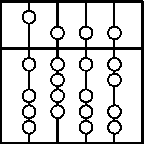
\includegraphics[width=2.4cm]{tum-abakus}

\end{center}

\newpage

%%%%%%%%%%%%%%%%%%%%%%%%%%%%%%%
% zweite Seite

\thispagestyle{empty}
\cleardoublepage 

%%%%%%%%%%%%%%%%%%%%%%%%%%%%%%%
% dritte Seite

\thispagestyle{empty}

\begin{center}


\includegraphics[width=3cm]{tum-logo}

\vspace{1cm}

{\Huge FAKULT�T F�R INFORMATIK\\[1mm]}
DER TECHNISCHEN UNIVERSIT�T M�NCHEN\\

\vspace{2cm}

{\Large \textbf{\typeOfThesis\ in Informatik}}\\

\vspace{2.0cm}
{\Huge \textbf{\titleOfThesisOne}}\\
\vspace*{3mm}
{\Huge \textbf{\titleOfThesisTwo}}\\
\vspace*{3mm}
{\Huge \textbf{\titleOfThesisThree}}\\

\vspace{1.5cm}

\parbox{1cm}{
  \begin{large}
    \begin{tabbing}
      Bearbeiter: \hspace{1cm}
        \=\authorOfThesis\\[2mm]
      Aufgabensteller:
        \>\aufgabensteller\\[2mm]
      Betreuer: 
        \>\betreuerOne\\
        \>\betreuerTwo\\
      Abgabedatum: 
        \> \abgabeTagZahl.~\abgabeMonatText~\abgabeJahrZahl\\
    \end{tabbing}
  \end{large}
}\\

\vspace{5mm}

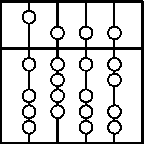
\includegraphics[width=2.4cm]{tum-abakus}

\end{center}
%
  \fi%
  \ifLMU%
    %%
% LaTeX-Rahmen f�r Arbeiten am Lehrstuhl Hegering
%
% Harald Roelle, 2001, 2002
%
% basierend auf Arbeiten von Helmut Reiser, Boris Gruschke und Stephen Heilbronner
%


%Link im PDF
\ifpdf
  \pdfbookmark[0]{Titel}{Titel}%
\fi

%%%%%%%%%%%%%%%%%%%%%%%%%%%%%%%
% erste Seite

\thispagestyle{empty}

\begin{center}

\vspace*{-2cm}

{\Huge INSTITUT F�R INFORMATIK\\[1mm]}
DER LUDWIG--MAXIMILIANS--UNIVERSIT�T M�NCHEN\\

\vspace*{1cm}


\includegraphics[width=0.3\textwidth]{lmu_siegel}

\vspace*{2cm}

{\Large \textbf{\typeOfThesis}}\\

\vspace{2.0cm}
{\Huge \textbf{\titleOfThesisOne}}\\
\vspace*{3mm}
{\Huge \textbf{\titleOfThesisTwo}}\\
\vspace*{3mm}
{\Huge \textbf{\titleOfThesisThree}}\\

\vspace{1.5cm}

{\LARGE \authorOfThesis}

%\vspace{2cm}

%\parbox{1cm}{
%  \begin{large}
%    \begin{tabbing}
%      Aufgabensteller:
%        \=\aufgabensteller\\[2mm]
%      Betreuer: 
%        \>\betreuerOne\\
%        \>\betreuerTwo\\
%        \>\betreuerThree\\[5mm]
%      Abgabetermin: 
%        \> \abgabeTagZahl.~\abgabeMonatText~\abgabeJahrZahl\\
%    \end{tabbing}
%  \end{large}
%}\\

\end{center}

\newpage

%%%%%%%%%%%%%%%%%%%%%%%%%%%%%%%
% zweite Seite

\thispagestyle{empty}
\cleardoublepage 

%%%%%%%%%%%%%%%%%%%%%%%%%%%%%%%
% dritte Seite (Kopie der ersten)

\thispagestyle{empty}

\begin{center}

\vspace*{-2cm}

{\Huge INSTITUT F�R INFORMATIK\\[1mm]}
DER LUDWIG--MAXIMILIANS--UNIVERSIT�T M�NCHEN\\

\vspace*{1cm}


\includegraphics[width=0.3\textwidth]{lmu_siegel}

\vspace*{2cm}

{\Large \textbf{\typeOfThesis}}\\

\vspace{2.0cm}
{\Huge \textbf{\titleOfThesisOne}}\\
\vspace*{3mm}
{\Huge \textbf{\titleOfThesisTwo}}\\
\vspace*{3mm}
{\Huge \textbf{\titleOfThesisThree}}\\

\vspace{1.5cm}

{\LARGE \authorOfThesis}

\vspace{2cm}

\parbox{1cm}{
  \begin{large}
    \begin{tabbing}
      Aufgabensteller:
        \=\aufgabensteller\\[2mm]
      Betreuer: 
        \>\betreuerOne\\
        \>\betreuerTwo\\
        \>\betreuerThree\\[5mm]
      Abgabetermin: 
        \> \abgabeTagZahl.~\abgabeMonatText~\abgabeJahrZahl\\
    \end{tabbing}
  \end{large}
}\\

\end{center}
%
  \fi%
  
  % Erkl�rung
  %\input{erklaerung}%
  
  % Abstract
  %\begin{DAabstract}%
  %  Hier steht eine kurze Zusammenfassung der Arbeit. Sie darf auf gar keinen Fall 
l�nger als eine Seite sein, ca. eine  halbe Seite ist optimal.

Das Abstract muss einfacher Plain-Text sein mit Leerzeile f�r Abs�tze. 
Grund: Daraus l�sst sich dann einfach der HTML-Text erzeugen, der automatisch
auf der Web-Page erscheint.
%
  %\end{DAabstract}%

  \pagestyle{empty}%
  \pagenumbering{roman}%
}

%
% �bergang von Verzeichnissen zum Hauptteil
%
\newcommand{\setupMainPart}[0]{%
  \cleardoublepage%
  \pagestyle{headings}%
  \pagenumbering{arabic}%
}

%
% Anh�nge
%
\newcommand{\appendixbegin}[0]{%
  \cleardoublepage%
  \begin{appendix}%
  \setcounter{secnumdepth}{3}%
}
\newcommand{\appendixend}[0]{%
  \end{appendix}%
  \cleardoublepage%
}

%
% Wrapper fuer Literaturverzeichnis
%
\newcommand{\listofreferences}[0]{%
  \cleardoublepage%
  \bibliographystyle{geralpha-mnm-0.2} % Zitierungs-Richtlinien des Lehrstuhls
  \bibliography{\bibfiles}%
}

%
% Wrapper fuer Dokumentende
%
\newcommand{\docend}[0]{%
  \end{document}
}


%%% Local Variables: 
%%% mode: latex
%%% TeX-master: t
%%% End: 
